\documentclass{beamer}

\usetheme[]{Rochester}
\usecolortheme{beaver}
\usepackage[latin1]{inputenc}
\usepackage{graphics}

\author{Will Webberley}
\date{Autumn 2014}
\institute[COMSC]{Cardiff School of Computer Science and Informatics}



\title{Cognitive Evaluation}
\subtitle{CM2101: Human-Computer Interaction}

\begin{document}

\frame{\titlepage}

\frame{
    \frametitle{Cognitive evaluation}
    \center{
        It is important to consider the \alert{cognitive demands} of users.
    }
    \vskip20pt
    \flushleft{
        Cognitive evaluation allows us to
        \begin{itemize}
            \item Consider the users' \alert{working memories}
            \item \alert{Compare} methods of carrying out tasks within a system
            \item Itemize the \alert{subtasks} involved in carrying out a task
        \end{itemize}
    }
}

\frame{
    \frametitle{Cognitive evaluation}
    \begin{columns}
        \column{.5\textwidth}
            \begin{itemize}
                \item Useful in collaboration with \alert{user} and \alert{heuristic} evaluation 
                \item Useful in the \alert{evaluation} phase of the iterative design cycle
                \item Highlights a user's \alert{cognitive perception} of a task  
                \item Useful in systems with different software interfaces
                \item Useful in systems with different hardware interfaces
                \item Based on human psychology
            \end{itemize}
        \column{.5\textwidth}
            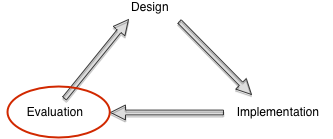
\includegraphics[width=5cm]{media/cycle_2.png}
    \end{columns}
}

\frame{
    \frametitle{Humans in task analysis}
    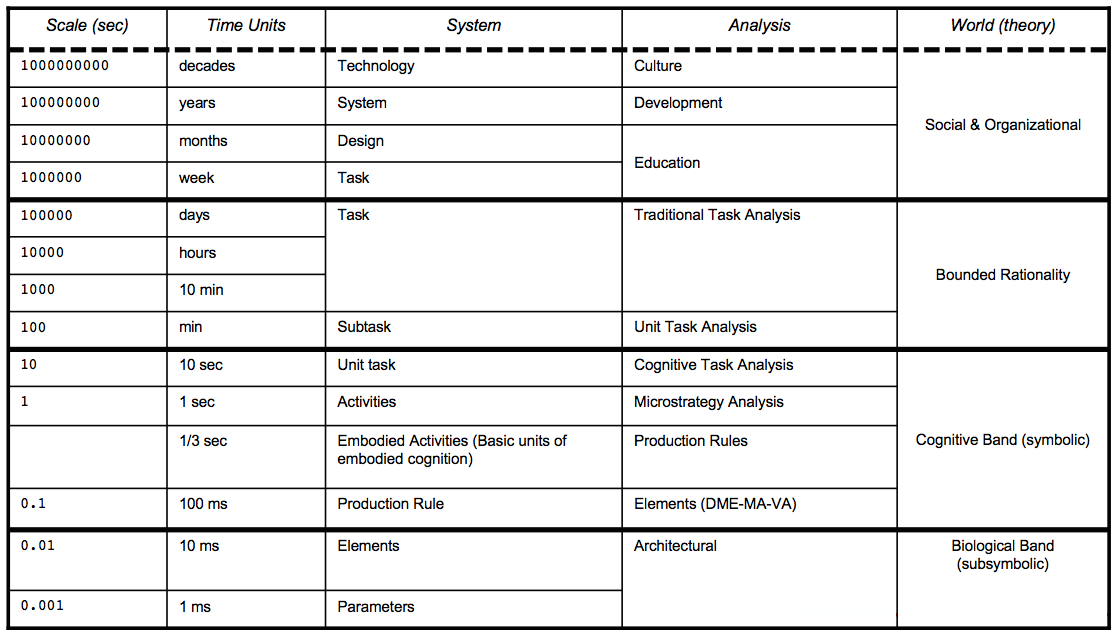
\includegraphics[width=\textwidth]{media/big_table.png}
}
    
\frame{
    \frametitle{Cognitive modelling}
    \textbf{We will consider two types of cognitive modelling}
    \vskip20pt
    \begin{itemize}
        \item GOMS
        \begin{itemize}
            \item \textbf{G}oals, \textbf{O}perators, \textbf{M}ethods, and \textbf{Selections}
            \item Models task \alert{acquisition} - how a user goes about completing a task
            \item Developed by Card, Moran, and Newell
        \end{itemize}
        \vskip20pt
        \item KLM
        \begin{itemize}
            \item \textbf{K}eystroke-\textbf{L}evel \textbf{M}odel
            \item Models task \alert{execution} - how the available facilities are used to complete the task
            \item Developed by David Kieras
            \item Perhaps more useful on traditional keyboard+mouse systems
        \end{itemize}
    \end{itemize}
}

\frame{
    \frametitle{GOMS}
    \textbf{Attempts to model a user's thought processes}
    \begin{itemize}
        \item \alert{Goals} - The state the user wants to achieve
        \begin{itemize}
            \item e.g. finding a particular screen of an app or carrying out a particular task
        \end{itemize}
        \item \alert{Operators} - Cognitive processes \& physical actions needed to reach the state
        \begin{itemize}
            \item e.g. which buttons to press or controls to use to achieve the state
        \end{itemize}
        \item \alert{Methods} - Granular procedures for accomplishing sub-goals
        \begin{itemize}
            \item e.g. move finger over field, tap field, type in word, move finger to button, tab button
        \end{itemize}
        \item \alert{Selections} - Rules for determining the best route to achieve the state (if there is more than one)
        \begin{itemize}
            \item e.g. is it less cognitively demanding to use a keyboard shortcut to close a browser tab or move the mouse to the close button?
        \end{itemize}
    \end{itemize}
}

\frame{
    \frametitle{GOMS}
    \center{
        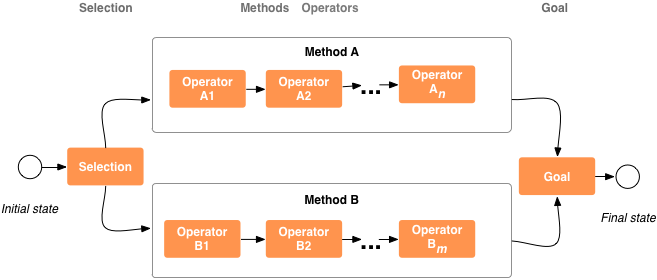
\includegraphics[width=\textwidth]{media/goms.png}
    }
}

\frame{
    \frametitle{GOMS}
    \center{
        We want to represent users' \alert{knowledge}, \alert{understanding}, and \alert{intentions}.
    }
    \flushleft{
        \begin{itemize} 
            \item A form of task analysis (we'll cover this more soon...)
            \item How does the user formulate goals?
            \item What does the user have to remember in the short term?
            \item What does the user have to remember in the long term?
            \item How does the user translate intentions into actions?
        \end{itemize}
    }
}

\frame{
    \frametitle{GOMS example}
    \begin{columns}
        \column{.5\textwidth}
        \begin{block}{Example overview}
            \begin{description}[Platform]
                \item[Platform] Alarm clock (hardware)
                \item[Task] Set the time
                \item[Result] Time has been set
            \end{description}
        \end{block}
        \column{.5\textwidth}
            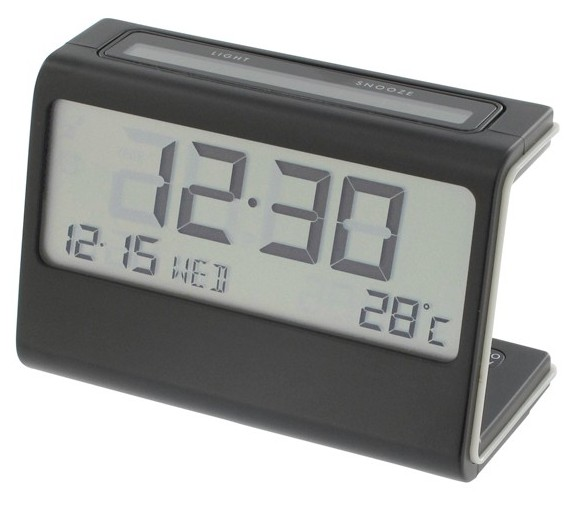
\includegraphics[width=5cm]{media/clock.jpg}
    \end{columns}
}

\frame{
    \frametitle{GOMS example}
    \textbf{\alert{Stage 1}: Identify goals and subgoals}
    \vskip20pt
    \begin{columns}
        \column{.5\textwidth}
            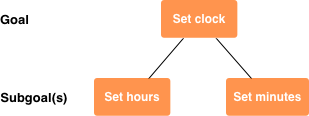
\includegraphics[width=6cm]{media/goms_goals.png}
        \column{.5\textwidth}
            \begin{itemize}
                \item Try and break the main goal down into a series of sub-goals
                \item This is the trickiest part (as it can be quite vague)
            \end{itemize}
    \end{columns}
}

\frame{
    \frametitle{GOMS example}
    \textbf{\alert{Stage 2}: Identify operators}
    \vskip20pt
    \begin{columns}
        \column{.5\textwidth}
            \begin{block}{Operators}
                \begin{itemize}
                    \item Click button \texttt{<button>}
                    \item Depress button \texttt{<button>}
                    \item Release button \texttt{<button}
                    \item Decide if \texttt{<X>}, then \texttt{<Y>}
                    \item Wait for \texttt{<X>}
                \end{itemize}
            \end{block}
        \column{.5\textwidth}
            \begin{itemize}
                \item List all of the operators required in this task
                \item These are the most elementary steps used to carry out a task 
            \end{itemize}
    \end{columns}
}

\frame{
    \frametitle{GOMS example}
    \textbf{\alert{Stage 3}: Identify methods}
    \vskip20pt
    \begin{block}{Methods}
        \begin{itemize}
            \item Top-level goal
            \begin{enumerate}
                \item Complete goal: \texttt{SET\_CLOCK}
            \end{enumerate}
            \vskip10pt
            \item Method for goal: \texttt{SET\_CLOCK}
            \begin{enumerate}
                \item Depress button \texttt{time}
                \item Complete goal: \texttt{SET\_DIGIT(hour)}
                \item Complete goal: \texttt{SET\_DIGIT(minute)}
                \item Release button \texttt{time}
                \item Return with goal completed
            \end{enumerate}    
        \end{itemize}
    \end{block}
}

\frame{
    \frametitle{GOMS example}
    \textbf{\alert{Stage 3 contd.}: Identify methods}
    \vskip20pt
    \begin{block}{Methods contd.}
        \begin{itemize}
            \item Method for goal: \texttt{SET\_DIGIT(type)} 1
            \begin{enumerate}
                \item Click button \texttt{type}
                \item Decide if \texttt{current digit = target digit} then 
                \begin{itemize}
                    \item Return with goal completed
                \end{itemize}
                \item Goto \texttt{step 1}
            \end{enumerate}
            \item Method for goal: \texttt{SET\_DIGIT(type)} 2
            \begin{enumerate}
                \item Depress button \texttt{type}
                \item Wait for \texttt{current digit = target digit}
                \item Release button \texttt{type}
                \item Return with goal completed
            \end{enumerate}
        \end{itemize}   
    \end{block}
}

\frame{
    \frametitle{GOMS example}
    \textbf{\alert{Stage 4}: Make selection rules}
    \vskip20pt
    How do we choose between the two \texttt{SET\_DIGIT} methods?
    \vskip10pt
    \begin{block}{Selection rules}
        Selection rule for \texttt{SET\_DIGIT}
        \begin{itemize}
            \item If \texttt{current digit < (target digit - 4)}
            \begin{itemize}
                \item Use method \texttt{2}
            \end{itemize}
            \item Else
            \begin{itemize}
                \item Use method \texttt{1}
            \end{itemize}
        \end{itemize}
    \end{block}
}

\frame{
    \frametitle{GOMS addressing cognition}
    Human working memory:
    \begin{itemize}
        \item Small (~7 individual `chunks')
        \item short-lived (~10 seconds)
        \item Neilsen's \textit{Recognition vs. recall} heuristic helps address this
    \end{itemize}
    \vskip20pt
    How is GOMS useful?
    \begin{itemize}
        \item `Depth' of goal structure can estimate working memory requirement
        \item The more sub-goals to achieve, the larger the cognitive burden
        \item Users might forget what their primary goal is if there are many sub-goals
    \end{itemize}
}

\frame{
    \frametitle{GOMS summary}
    What can GOMS do?
    \begin{itemize}
        \item Help predict the sequence of operators a person will use to complete a goal
        \item Help predict \textit{Learnability}
        \item Help preduct savings due to previous learning
        \item Help produce guides and documentation
    \end{itemize}
}

\frame{
    \frametitle{GOMS summary}
    What can't GOMS do?
    \begin{itemize} 
        \item Predict behavious of casual users
        \item Predict individual differences
        \item Predict the effects of fatigue and individual preferences
    \end{itemize}
}

\frame{
    \frametitle{Suggestions from GOMS}
    \begin{itemize}
        \item If selection rules cannot easily be defined, then you may need to eliminate redundant methods
        \item Increase efficiency for common tasks by designing shorter methods (or shortcuts)
        \item Reduce learning time by combining or eliminating methods
        \item Complex tasks can take longer than many shorter sub-tasks, due to required mindpower
    \end{itemize}
}   

\frame{
    \frametitle{KLM}
    \textbf{Extension of GOMS for predicting how long a task might take}
    \begin{itemize}
        \item Use operators derived from GOMS to predict a completion \alert{time}
        \item Typically more useful on traditional keyboard+mouse systems...
        \item ... though apliccable in principle to any interactive system
        \item Aimed at \alert{short tasks} in interaction (about $<$ 20 seconds)
        \begin{itemize}
            \item e.g. `Copy+paste', `change font', but \textbf{not} `edit document'       
        \end{itemize}
        \item Goals or selection rules not considered - only operators and methods
        \item Allows \alert{comparisons} between different design options
        \item KLM assumes that the user is \alert{expert}
    \end{itemize}
}

\frame{
    \frametitle{KLM}
    \textbf{KLM modelling}
    \begin{itemize}
        \item KLM considers 
        \begin{itemize}
            \item Description of the task (through the `operators')
            \item Simple model of a user
            \item Simple model of a computer 
        \end{itemize}
        \item Predicting time:
        \begin{itemize}
            \item Time to complete a task ($x$) is the sum of the time taken to carry out each operator
            \item $T_x = T_k + T_b + T_p + T_h + T_d + T_m + T_r$
        \end{itemize}
    \end{itemize}
}

\frame{
    \frametitle{KLM}
    \textbf{Time for operators} (\textit{Dix et al})\\
    \vskip10pt
    \begin{tabular}{| c | l | l | r |}
        \hline
        \textbf{Operator} & \textbf{Action} & \textbf{Action info} & \textbf{Time (sec.)}\\
        \hline
        \hline
        K & Press key & Good typist & 0.12\\
        & & Poor typist & 0.28\\
        \hline
        B & Mouse button & Press or release & 0.10\\
        & & click & 0.20\\
        \hline
        P & Point & mouse or finger & 1.10\\
        \hline
        H & `Home' hands &  & 0.40\\
        \hline
        M & Mentally prepare & & 1.35\\
        \hline
        R & Response time & System-dependent & $t$\\
        \hline 
    \end{tabular}
}

\frame{
    \frametitle{KLM: when to add Ms?}
    \begin{itemize}
        \item Not required before \textit{every} operator
        \item Only before a group of operators that need to be recalled from long-term memory
        \vskip20pt
        \item Before each sub-goal (but also long operators)
        \item When deciding on the way to do a task
        \item When finding something on a screen
        \begin{itemize}
            \item Thus \textit{P} usually preceeded by M
        \end{itemize}
        \item When verifying input or action result
        \begin{itemize}
            \item e.g. before pressing `OK' on a dialog
        \end{itemize} 
    \end{itemize}
}

\frame{
    \frametitle{KLM example}
    \begin{itemize}
        \item Usually, KLM would be done after GOMS modelling...    
        \item ... as GOMS would identify the list of operations needed to complete a goal
        \item However, here we will just use a simple example
    \end{itemize}        
}

\frame{
    \frametitle{KLM example}
    \begin{block}{Example overview}
        \begin{description}[Assumptions]
            \item[Goal] Search for `human-computer interaction' on Google
            \item[Platform] Desktop machine with keyboard+mouse
            \item[Assumptions] 
                \begin{itemize}
                    \item Simple browser (no auto-complete, searching from an omnibox, etc.)
                    \item Browser is already open
                    \item Address bar is empty
                    \item Our identified method is the only one
                    \item User is a `good typist'
                \end{itemize}
        \end{description}
    \end{block}
}
        
\frame{
    \frametitle{KLM example}
    \textbf{Methods found in GOMS analysis} 
     \vskip20pt
     \begin{block}{Methods and operators}
         \begin{itemize}
             \item Top-level goal
             \begin{enumerate}
                 \item Complete goal: \texttt{SEARCH\_GOOGLE(term)}
             \end{enumerate}
             \vskip10pt
             \item Method for goal: \texttt{SEARCH\_GOOGLE(term)}
             \begin{enumerate}
                \item Move cursor to address bar
                \item Click mouse 
                \item Enter \texttt{www.google.co.uk}
                \item Press \texttt{return} key
                \item Wait for \texttt{the page at www.google.co.uk to load}                
                \item Move cursor to search textfield
                \item Enter \texttt{term}
                \item Press \texttt{return key}
                \item Return with goal completed
             \end{enumerate}    
         \end{itemize}
     \end{block}
}             

\frame{
    \frametitle{KLM example}
    \textbf{KLM analysis of identified operators}
    \vskip10pt
    \begin{block}{KLM analysis}
        \begin{description}[Move mouse and click]
            \item[Initial homing] $T_h$
            \item[Move mouse and click] $T_m + T_p + T_b$ 
            \item[Enter text] $T_m + (16 * T_k)$
            \item[Verify \& press enter] $T_m + T_k$
            \item[System wait] $T_r$
            \item[Move mouse and click] $T_m + T_p + T_b$
            \item[Enter text] $T_m + (23 * T_k)$
            \item[Verify \& press enter] $T_m + T_k$ 
        \end{description}
        $T_x = 0.4 + 2.65 + 3.27 + 1.47 + T_r + 2.65 + 4.11 + 1.47$
        $T_x = 16.02 + T_r$  
    \end{block}
}

\frame{
    \frametitle{GOMS + KLM summary}
    \textbf{Advantages}
    \vskip20pt
    \begin{itemize}
        \item Can be used on low-fidelity prototypes near start of iterative cycle
        \item Methods can be prepared before any implementation
        \item Generally, not necessary to use more than one expert evaluator
        \item The theory provides explanation
        \begin{itemize}
            \item User testing may \textit{reveal} problems, but might not \textit{explain} them 
        \end{itemize}
    \end{itemize}
}

\frame{
    \frametitle{GOMS + KLM summary}
    \textbf{Disadvantages}
    \vskip20pt
    \begin{itemize}
        \item Is time to do a task \textit{always} the most useful performance metric?
        \item Generally only measures \textit{Efficiency} and not things like \textit{Consistency}, \textit{Errors}, etc.
        \item Based only on \alert{expert users} - is this reasonable?
        \item Both GOMS and KLM ignore:
        \begin{itemize}
            \item Errors that may occur
            \item Parallel actions (e.g. multi-touch or shift-clicking)
            \item Planning and problem-solving (i.e. doesn't actually help the end user - how do they select the method?)
        \end{itemize}
    \end{itemize}
}

\frame{
    \frametitle{Revision questions}
    \begin{enumerate}
        \item What does cognitive modelling allow designers to achieve?
        \item At what stage are GOMS and KLM useful in interactive system design?
        \item Describe GOMS and give a brief overview of what it models.
        \item What does the `selections' stage of GOMS modelling refer to?
        \item What are the benefits of GOMS modelling?
        \item Describe KLM and explain what it is useful for.
        \item Name three operators that KLM considers. 
    \end{enumerate}
    In the exam, you may be asked to carry out GOMS/KLM modelling on a given example system, but you will \textit{not} be expected to remember operation times for KLM.
}

\frame{
    \frametitle{Summary}
    \begin{itemize}
        \item Overview of cognitive evaluation and modelling
        \item Introduction to GOMS modelling
        \item Introduction to KLM modelling
        \item Practical examples of using GOMS and KLM modelling        
    \end{itemize}
}    




\end{document}
